\newacronym{prbs}{PRBS}{\textit{Pseudo-Random Binary Signal}}
\newacronym{arma}{ARMA}{\textit{Auto-Regressive Moving Average}}
\newacronym{gbn}{GBN}{\textit{Generalized Binary Noise}}
\newacronym{ar}{AR}{modelo autorregressivo}
\newacronym{arx}{ARX}{modelo autorregressivo com entrada exógena}
\newacronym{armax}{ARMAX}{modelo autorregressivo com média móvel e entrada exógena}

\chapter{Metodologia}
\label{ch:metodologia}

% =====================================================================================================
% ============================================= Section ===============================================
% =====================================================================================================
\section{Modelagem experimental}
\label{sec:modelagem_experimental}

Segundo \citeonline{Gevers2006} a teoria de identificação de sistemas data da década de 60 e as duas
principais técnicas utilizadas na identificação de sistemas atualmente (método de identificação por
subespaço de estados e método do erro de predição) tiveram suas bases estruturadas com os trabalhos
de \apudonline{Ho1966}{Gevers2006} e de \apudonline{Astrom1965}{Gevers2006}.

De acordo com \apudonline{Dunia2008}{Pracek2012} a identificação do sistema permite que simulações
sejam desenvolvidas de modo a garantir um melhor desempenho dos sistemas de controle projetados.

As etapas para a identificação de um sistema, segundo \citeonline{Aguirre2015} são:
\begin{itemize}
    \item Testes dinâmicos e coleta de dados
    \item Escolha da representação matemática a ser utilizada
    \item Determinação da estrutura do modelos
    \item Estimação de parâmetros
    \item Validação do modelo
\end{itemize}

As seções a seguir detalham cada uma dessas etapas.

% .....................................................................................................
% ............................................ Subsection .............................................
% .....................................................................................................
\subsection{Testes dinâmicos e coleta de dados}
\label{subsec:testes_dinamicos_e_coleta_de_dados}

Esta etapa abrange os procedimentos necessários para geração do conjunto de dados que serão utilizados
para a identificação do sistema. Algumas das atividades realizadas nessa etapa são: escolha das variáveis,
definição dos sinais de excitação, definição do período de amostragem e a execução em si dos testes.
\cite{Aguirre2015}

% -----------------------------------------------------------------------------------------------------
% ------------------------------------------- Subsubsection -------------------------------------------
% -----------------------------------------------------------------------------------------------------
\subsubsection{Período de amostragem}
\label{subsubsec:periodo_de_amostragem}

Segundo o teorema de Shannon, descrito por \citeonline{Aguirre2015}, "um sinal que não contenha componentes
de frequência acima de $1/2T_s$ pode ser determinado unicamente a partir de amostras de tal sinal separadas
por $T_s$", sendo $T_s$ o período de amostragem ou, como também é chamado, tempo de amostragem.

Na prática, contudo, um período de amostragem apenas 2 vezes maior que a frequência de interesse, como exigido
pelo teorema de Shannon, nem sempre é suficiente. Normalmente então escolhe-se uma frequência de amostragem
entre 5 e 10 vezes maior do que a maior do que tal frequência desejada \cite{Aguirre2015}. Por outro lado, do
ponto de vista numérico, se o intervalo de amostragem for muito curto, a estimação de parâmetros também
poderá se tornar malcondicionada \cite{Aguirre2015}.

Para a identificação da maior frequência de interesse do sistema analisado, alguns ensaios foram realizados\footnote{
    Indicar scripts utilizados          % TODO Indicar scripts utilizados
}
excitando o Aquecedor 1 do \acrshort{tclabsp} em $50\%$ e aproximando a resposta em malha aberta dos
Sensores de Temperatura 1 e 2 para um sistema de primeira ordem, a fim de obter o valor do tempo de subida
($\tau$). Esse tempo de subida servirá de referência para o cálculo do período de amostragem.

\begin{figure}[h]
	\caption{Tempo de subida - Sensor de Temperatura 1}
	\begin{center}
		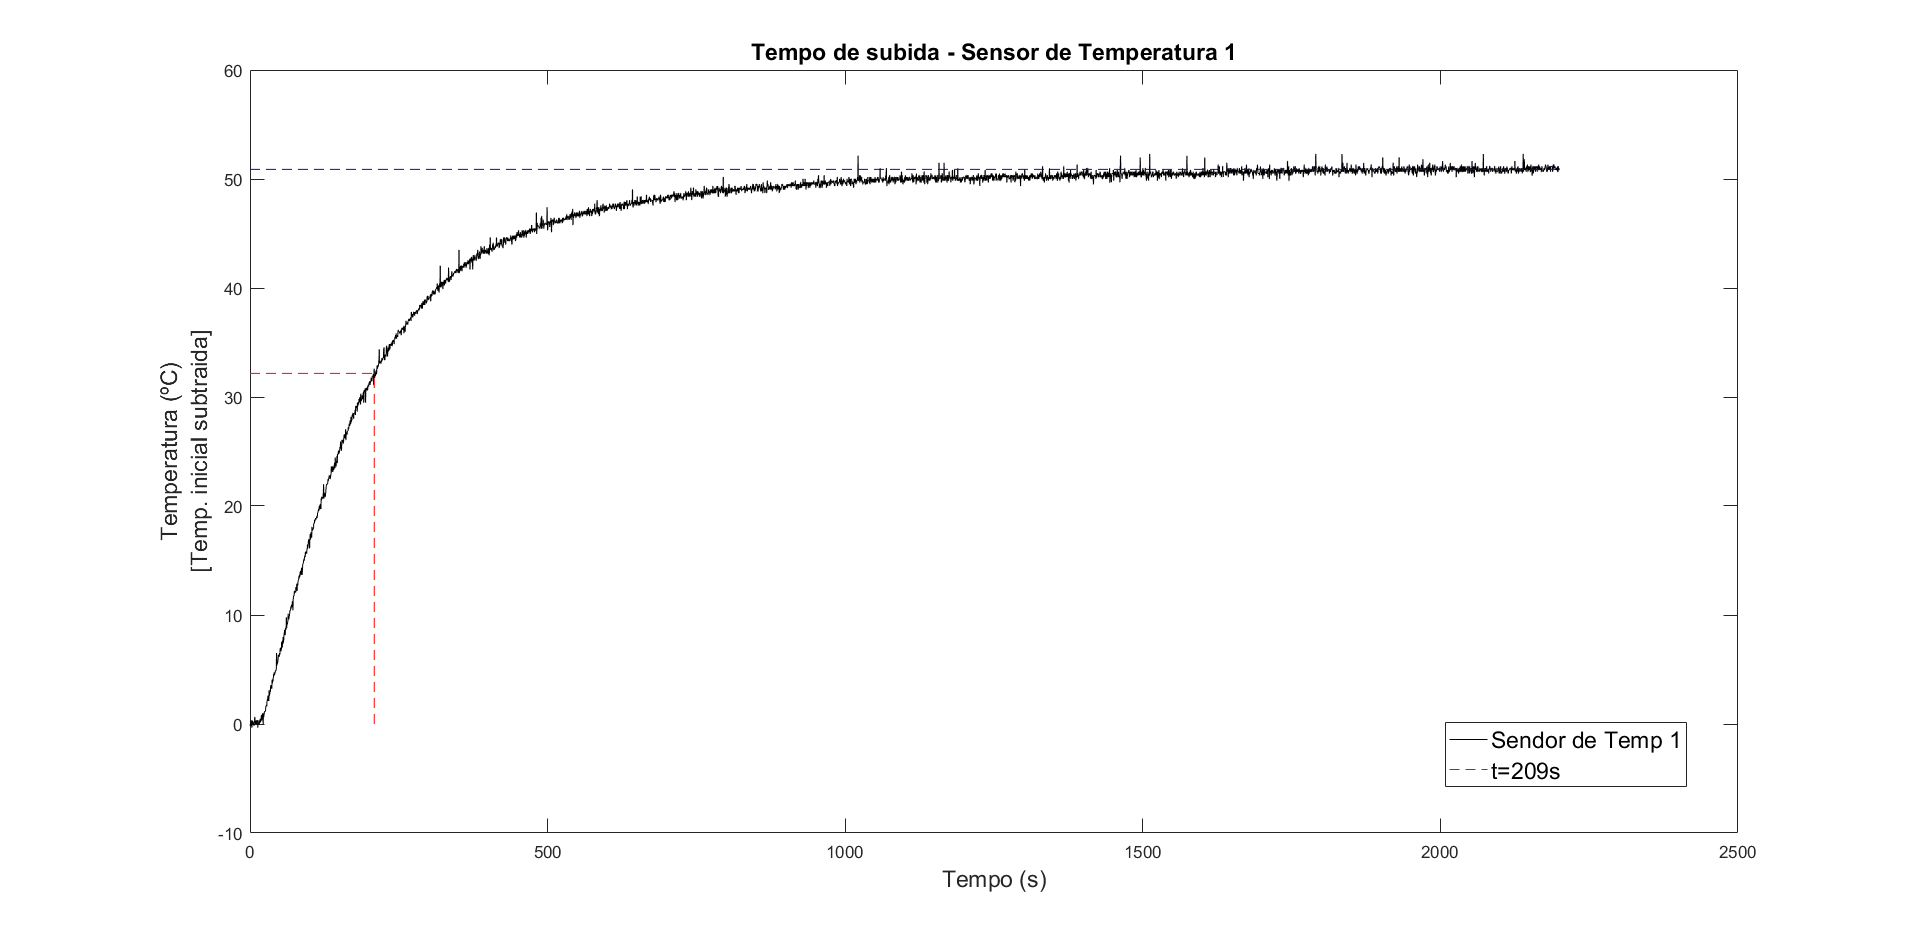
\includegraphics[width=0.85\textwidth]{./5_images/RiseTime-TempSensor1.png} 
		\label{fig:rise_time_sensor1}
	\end{center}
	\centering
	\makebox[\width]{Fonte: \citeonline{Prata2019}} 
\end{figure}

\begin{figure}[h]
	\caption{Tempo de subida - Sensor de Temperatura 1}
	\begin{center}
		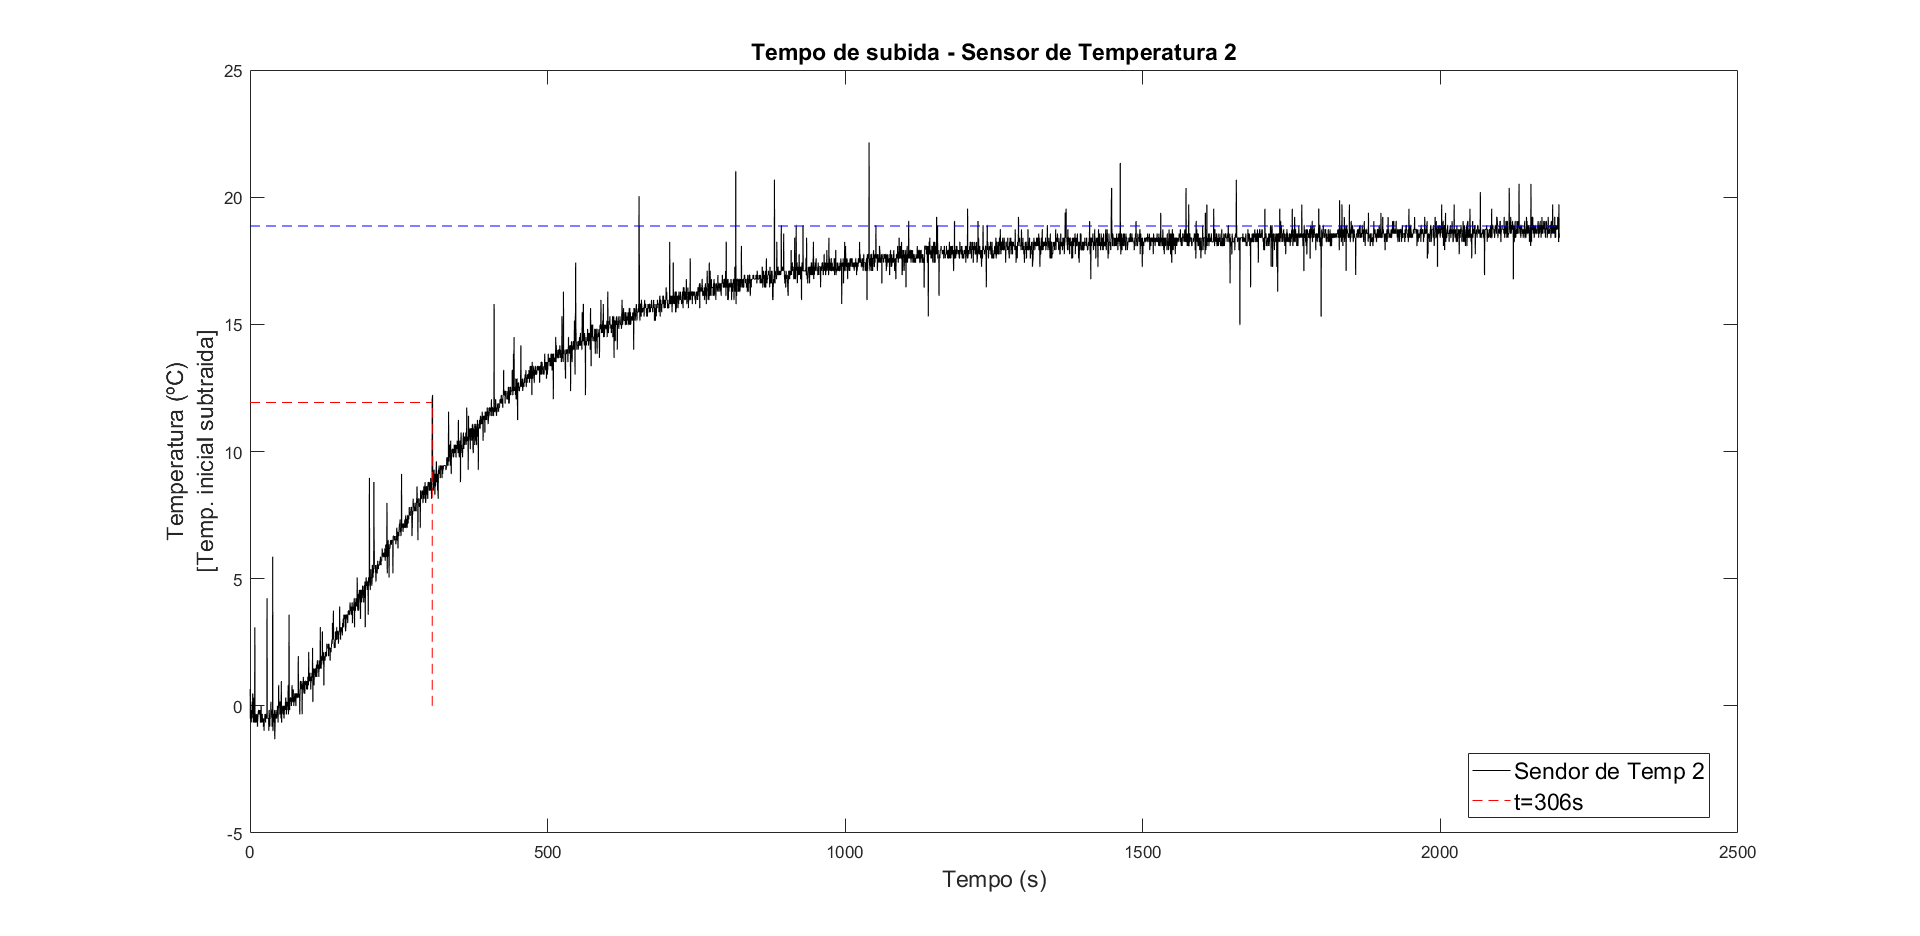
\includegraphics[width=0.85\textwidth]{./5_images/RiseTime-TempSensor2.png} 
		\label{fig:rise_time_sensor2}
	\end{center}
	\centering
	\makebox[\width]{Fonte: \citeonline{Prata2019}} 
\end{figure}

As \cref{fig:rise_time_sensor1,fig:rise_time_sensor2} mostram a resposta em malha aberta dos Sensores de
Temperatura 1 e 2, respectivamente, a uma entrada degrau no Aquecedor 1. Este ensaio foi realizado com
um período de amostragem de 0,5s, e com ele foi possível observar um tempo de subida $\tau_1 = 209s$ para
o Sensor 1 e $\tau_2 = 306s$ para o Sensor 2.
% TODO: Fazer mais ensaios com step 0 -> 50
% TODO: Recortar as imagens para remover bordas brancas

Seguindo a regra prática de \citeonline{Aguirre2015} onde $T_s$ deve ser entre 5 e 10 vezes maior que a
maior frequência desejada, então temos que $20.9s > T_s > 41.8s$.

Para os ensaios realizados neste trabalho, optou-se pela maior frequência de amostragem possível, como
mostrado na \cref{eq:sampling_time}.

\begin{equation}
	\label{eq:sampling_time}
	T_s = 20.9s
\end{equation}

Outra técnica também descrita por \citeonline{Aguirre2015} para a escolha da frequência de amostragem,
apesar de não ter sido escolhida, também foi testada e é descrita em maiores detalhes no
\cref{ch:sampling_time_using_autocorrelation}.

% -----------------------------------------------------------------------------------------------------
% ------------------------------------------- Subsubsection -------------------------------------------
% -----------------------------------------------------------------------------------------------------
\subsubsection{Sinais de excitação}
\label{subsubsec:sinais_de_excitacao}

% \acrshort{arma} - Média Móvel Auto-Regressiva (do inglês, \acrlong{arma})
A escolha dos sinais de entrada pode ter grande impacto nos dados coletados,
pois determinarão o ponto de operação do sistema e quais das suas características serão excitadas
durante o experimento \cite{Aguirre2015}.
Diversos tipos distintos de sinais podem ser utilizados. Entre os mais comuns destacam-se:
impulsivo; degrau; \acrshort{prbs} - Sinal Binário Pseudo-Aleatório (do inglês, \acrlong{prbs});
\acrshort{gbn} - Ruido Binário Generalizado (do inglês, \acrlong{gbn}); soma de senóides e etc \cite{Aguirre2015}.
Porém quando objetiva-se a identificação do sistema de onde os dados foram coletados, no geral
os métodos de identificação exigem que os sinais de entrada tenham um espectro de frequência
branco ou quase branco. Sinais aleatórios e pseudoaleatórios satisfazem essa condição \cite{Aguirre2015}.

Sinais \acrshort{prbs} são comumente usados na identificação de sistemas lineares, porém para sistemas
não-lineares tais sinais não são adequados, neste caso muitas vezes será desejável excitar o
sistema numa larga faixa de amplitudes a fim de poder observar suas características estáticas e dinâmicas
\cite{Aguirre2015}.

\begin{citacao}
    Características dinâmicas e estáticas que não forem excitadas não aparecerão nos dados. O que
    não estiver nos dados não pode ser identificado. Tal princípio é utilizado, por exemplo,
    quando um sistema é excitado em torno de um ponto de operação. Neste caso, como as não-linearidades
    não foram excitadas no teste, é possível, pelo menos em princípio, ajustar um modelo linear
    aos dados assim obtidos. \cite{Aguirre2015}
\end{citacao}

Segundo \citeonline{Aguirre2015} uma regra prática para a aplicação do sinal de excitação é,
tendo-se definido o tempo de amostragem (já discutido na \cref{subsubsec:periodo_de_amostragem}),
manter constante o valor escolhido aleatóriamente por um tempo, em torno de 3 a 5 intervalos de
amostragem.

Para a coleta dos sinais do \acrshort{tclabsp} foram aplicados tanto no Aquecedor 1 quanto no
Aquecedor 2 sinais de entrada aleatórios, mantidos constantes por um período de $3T_s$ a $5T_s$
(vide \cref{eq:sampling_time}). Contudo, antes dos sinais aleatórios serem aplicados aos
aquecedores, um sinal constante de $50\%$ foi aplicado a cada um deles por $1500s$ com o intuito
de estabilizá-los em um patamar onde as amplitudes dos sinais aleatórios aplicados tivessem
maior liberdade. A \cref{fig:simulink_coleta} mostra o modelo \textit{Simulink} utilizado para
a coleta dos dados e a \cref{fig:experiment_inputs} mostra os sinais de entrada aplicados nos
Aquecedores 1 e 2.

\begin{figure}[h]
	\caption{Modelo \textit{Simulink} para coleta de dados}
	\begin{center}
		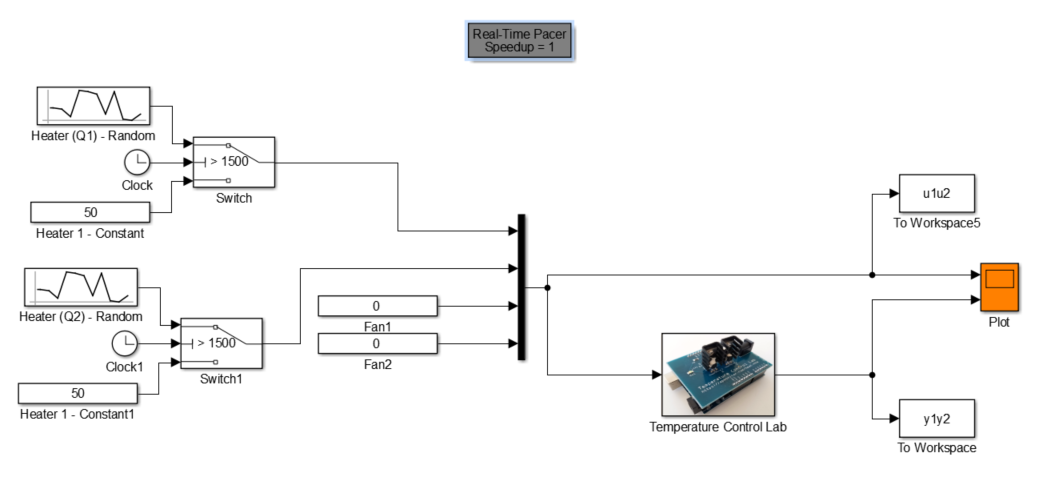
\includegraphics[width=0.85\textwidth]{./5_images/SimulinkColeta.png} 
		\label{fig:simulink_coleta}
	\end{center}
	\centering
	\makebox[\width]{Fonte: Autor} 
\end{figure}

\begin{figure}[h]
	\caption{Sinais de entrada nos Aquecedores 1 e 2}
	\begin{center}
		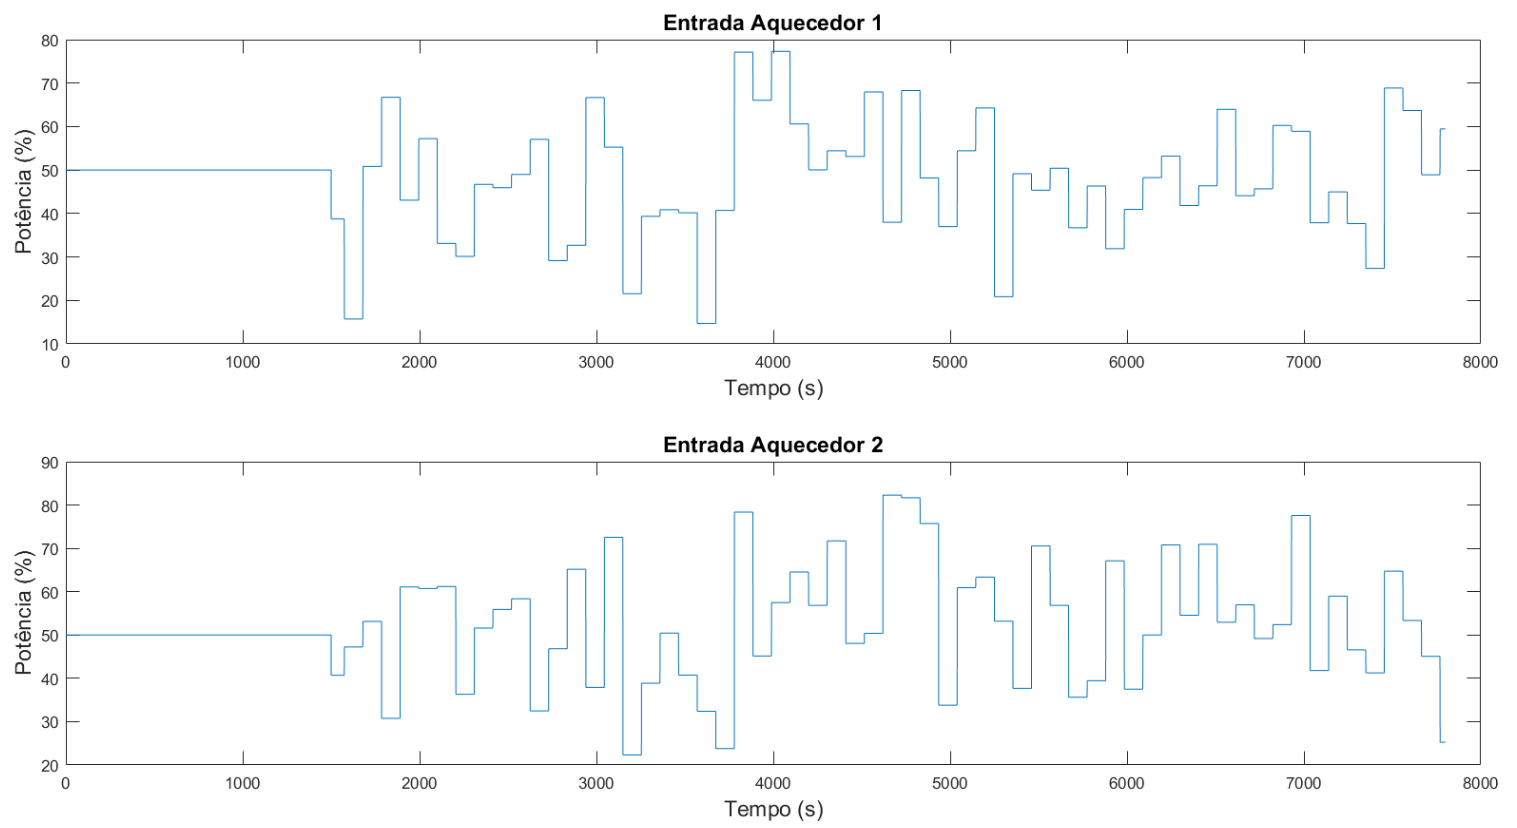
\includegraphics[width=0.85\textwidth]{./5_images/inputs_H1H2.png} 
		\label{fig:experiment_inputs}
	\end{center}
	\centering
	\makebox[\width]{Fonte: Autor} 
\end{figure}

% -----------------------------------------------------------------------------------------------------
% ------------------------------------------- Subsubsection -------------------------------------------
% -----------------------------------------------------------------------------------------------------
\subsubsection{Duração do experimento}
\label{subsubsec:duracao_do_experimento}

A duração do experimento, segundo \citeonline{Garcia2005}, deveria ser
a maior possível, uma vez que a variância das estimativas é proporcional ao inverso da duração do
experimento, porém sob o ponto de vista prático e experimental, a duração do experimento deveria ser
a menor possível para a obtenção de um modelo aceitável, pois ao longo do experimento o processo
estará sujeito a perturbações extras que podem impactar na operação da planta, na qualidade dos
produtos ou até na segurança do processo.

Cada um dos experimentos de coleta de dados do \acrshort{tclabsp} teve uma duração de $7800s$,
sendo que os $1500s$ iniciais foram utilizados para a estabilização do processo e os demais ($6300s$)
para as coletas. O critério utilizado para a determinação deste valor foi o de estimular a dinâmica
da planta aproximadamente $60x$ para cada um dos experimentos. Sabendo que os sinais de excitação
podem permanecer constantes por até $105s$ ($5T_s$), como mostrado na \cref{subsubsec:sinais_de_excitacao},
então temos a \cref{eq:experiment_duration}:

\begin{equation}
	\label{eq:experiment_duration}
	60 * 5T_s = \pmb{6}\pmb{3}\pmb{0}\pmb{0}\pmb{s}
\end{equation}

% .....................................................................................................
% ............................................ Subsection .............................................
% .....................................................................................................
\subsection{Escolha da representação matemática}
\label{subsec:escolha_da_representacao_matematica}

Existem diversas representações matemáticas distintas para modelos lineares, sendo que, segundo
\citeonline{Aguirre2015}, a mais utilizada é a função de transferência, porém \citeonline{Wang2009}
destaca que nos últimos anos tem se observado um aumento na popularidade dos modelos de espaço de
estados para desenvolvimento de controle preditivo. Para \citeonline{Aguirre2015} é importante ainda
salientar o modelo \acrshort{ar} (\acrlong{ar}), o modelo \acrshort{arx} (\acrlong{arx}) e
o modelo \acrshort{armax} (\acrlong{armax}).

\begin{citacao}
    \text{[...]} quando se trata da modelagem obtida por meios fenomenológicos é comum que se adote a base de
    tempo contínuo, em virtude de a maioria das leis da física serem expressas nesse tempo. Por sua vez,
    quando se trata de identificação de sistemas por processos experimentais, trabalha-se com amostras
    de dados coletados a cada intervalo de tempo, nesses casos usualmente adota-se o tempo discreto.
    \apud{Garcia2005}{Favaro2012}
\end{citacao}

% .....................................................................................................
% ............................................ Subsection .............................................
% .....................................................................................................
\subsection{Determinação da estrutura do modelos}
\label{subsec:determinacao_da_estrutura_do_modelo}

Determinar a ordem de um modelo é um dos aspectos mais importantes na determinação de sua estrutura,
uma vez que, caso sua ordem seja muito menor do que a ordem efetiva do sistema real, o modelo não
refletirá a completamente sua complexidade estrutural. Analogamente, escolher um modelo que a ordem
seja muito maior do que a necessária, provavelmente causará uma estimação de parâmetros mal condicionada.
\cite{Aguirre2015}

% .....................................................................................................
% ............................................ Subsection .............................................
% .....................................................................................................
\subsection{Estimação de parâmetros}
\label{subsec:estimacao_de_parametros}

A estimação de parâmetros, segundo \apudonline{Eykhoff1974}{Favaro2012} é a determinação experimental
de valores de parâmetros que governam a dinâmica e/ou o comportamento não-linear, assumindo que a
estrutura do modelo seja conhecida.

Essa etapa começa com a escolha do algoritmo a ser utilizado \cite{Aguirre2015}. Dentre eles, os
mais amplamente empregados na literatura são: método da análise de frequência; método da resposta
transitória e método dos mínimos quadrados \cite{Favaro2012}.

% .....................................................................................................
% ............................................ Subsection .............................................
% .....................................................................................................
\subsection{Validação do modelo}
\label{subsec:validacao_do_modelo}

Em problemas de validação, a questão é tentar determinar se um dado modelo é válido ou não e para isso,
deve-se simulá-lo sem qualquer ajuste adicional e compará-lo a dados medidos em testes diferentes daquele
usado no desenvolvimento da sintonia do mesmo. Ao se obter um conjunto de modelos, deve-se verificar se
eles incorporaram as características de interesse do sistema original \cite{Aguirre2015}.

\citeonline{Aguirre2015} em seu livro apresenta diversas ferramentas para auxiliar na validação dos modelos.

% =====================================================================================================
% ============================================= Section ===============================================
% =====================================================================================================
\section{Desenvolvimento do controlador}
\label{sec:desenvolvimento_do_controlador}

Através das \cref{eq:tclab_modelo_siso,eq:tclab_modelo_mimo_a,eq:tclab_modelo_mimo_b}
e também do modelo experimental que será obtido da planta piloto, utilizaremos a representação de
espaço de estados para a construção do modelo que irá compor os controladores.

Serão utilizadas duas abordagens principais:

\begin{itemize}
    \item \textbf{Utilização apenas de linguagens de programação, sem o auxílio de ferramentas de desenvolvimento
        \acrshort{mpc}}: esta abordagem tem como meta aplicar o controle \acrshort{mpc} através dos algoritmos
        descritos nas obras de \citeonline{Wang2009}, \citeonline{Rawlings2015}, \citeonline{Rossiter2003},
        entre outros, com a finalidade de detalhar cada etapa dos cálculos realizados pelo controlador
        visando cumprir os seguintes objetivos descritos na seção \ref{sec:objetivos}: estudo do algoritmo do
        controle \acrshort{mpc}; comparação entre a implementação em duas ou mais plataformas e compilação
        de material teórico e experimental sobre \acrshort{mpc}.
    \item \textbf{Utilização de ferramentas de desenvolvimento \acrshort{mpc}}: esta abordagem visa utilizar
        ferramentas consolidadas de mercado para o desenvolvimento de controlador \acrshort{mpc}, como o
        \textit{Model Predictive Control Toolbox}, disponível no \acrshort{matlab} para poder realizar
        a comparação entre o desempenho de um controlador \acrshort{mpc} em comparação a um controlador
        \acrshort{pid}, como também foi proposto nos objetivos da seção \ref{sec:objetivos}.
\end{itemize}